%%%%%%%%%%%%%%%%%%%%%%%%%%%%%%%%%%%%%%%%%
% Beamer Presentation
% LaTeX Template
% Version 1.0 (10/11/12)
%
% This template has been downloaded from:
% http://www.LaTeXTemplates.com
%
% License:
% CC BY-NC-SA 3.0 (http://creativecommons.org/licenses/by-nc-sa/3.0/)
%
%%%%%%%%%%%%%%%%%%%%%%%%%%%%%%%%%%%%%%%%%

%----------------------------------------------------------------------------------------
%	PACKAGES AND THEMES
%----------------------------------------------------------------------------------------

\documentclass{beamer}

\mode<presentation> {

% The Beamer class comes with a number of default slide themes
% which change the colors and layouts of slides. Below this is a list
% of all the themes, uncomment each in turn to see what they look like.

\usetheme{default}
%\usetheme{AnnArbor}
%\usetheme{Antibes}
%\usetheme{Bergen}
%\usetheme{Berkeley}
%\usetheme{Berlin}
%\usetheme{Boadilla}
%\usetheme{CambridgeUS}
%\usetheme{Copenhagen}
%\usetheme{Darmstadt}
%\usetheme{Dresden}
%\usetheme{Frankfurt}
%\usetheme{Goettingen}
%\usetheme{Hannover}
%\usetheme{Ilmenau}
%\usetheme{JuanLesPins}
%\usetheme{Luebeck}
%\usetheme{Madrid}
%\usetheme{Malmoe}
%\usetheme{Marburg}
%\usetheme{Montpellier}
%\usetheme{PaloAlto}
%\usetheme{Pittsburgh}
%\usetheme{Rochester}
%\usetheme{Singapore}
%\usetheme{Szeged}
%\usetheme{Warsaw}

% As well as themes, the Beamer class has a number of color themes
% for any slide theme. Uncomment each of these in turn to see how it
% changes the colors of your current slide theme.

%\usecolortheme{albatross}
%\usecolortheme{beaver}
%\usecolortheme{beetle}
%\usecolortheme{crane}
%\usecolortheme{dolphin}
%\usecolortheme{dove}
%\usecolortheme{fly}
%\usecolortheme{lily}
%\usecolortheme{orchid}
%\usecolortheme{rose}
%\usecolortheme{seagull}
%\usecolortheme{seahorse}
%\usecolortheme{whale}
%\usecolortheme{wolverine}

%\setbeamertemplate{footline} % To remove the footer line in all slides uncomment this line
%\setbeamertemplate{footline}[page number] % To replace the footer line in all slides with a simple slide count uncomment this line

%\setbeamertemplate{navigation symbols}{} % To remove the navigation symbols from the bottom of all slides uncomment this line
}

\usepackage{graphicx} % Allows including images
\usepackage{booktabs} % Allows the use of \toprule, \midrule and \bottomrule in tables

%----------------------------------------------------------------------------------------
%	CUSTOM TITLE PAGE COMMAND (can be called with \maketitle within the document)
%----------------------------------------------------------------------------------------

\defbeamertemplate*{title page}{customized}[1][]
{
	
	\usebeamercolor[fg]{titlegraphic}\inserttitlegraphic
	\usebeamerfont{title}\inserttitle\par
	\usebeamerfont{subtitle}\usebeamercolor[fg]{subtitle}\insertsubtitle\par
	\bigskip
	\usebeamerfont{author}\insertauthor\par
	\usebeamerfont{institute}\insertinstitute\par
	\bigskip
	\usebeamerfont{date}\insertdate\par
}

%----------------------------------------------------------------------------------------
%	TITLE PAGE ATTRIBUTES
%----------------------------------------------------------------------------------------

\title[Transformers]{Papers \& Cookies VII: Transformers} % The short title appears at the bottom of every slide, the full title is only on the title page
\subtitle{Vaswani et al.'s \textit{Attention Is All You Need}}

\author{Luis Oala} % Your name
\institute[ML Group @ Fraunhofer HHI] % Your institution as it will appear on the bottom of every slide, may be shorthand to save space
{
ML Group @ Fraunhofer HHI \\ % Your institution for the title page
%\medskip
%\textit{luis.oala@hhi.fraunhofer.de} % Your email address
}
\date{November 6, 2018} % Date, can be changed to a custom date

\titlegraphic{
\begin{figure}[t]
\includegraphics[width=0.65\textwidth]{figures/transformer_title.png}
\end{figure}
}

\begin{document}

%----------------------------------------------------------------------------------------
%	TITLE PAGE
%----------------------------------------------------------------------------------------
\begin{frame}

%\begin{figure}[t]
	%\includegraphics[width=0.5\textwidth]{figures/transformer_title.png}
%\end{figure}

\maketitle
	
\end{frame}
%----------------------------------------------------------------------------------------
%	OUTLINE
%----------------------------------------------------------------------------------------

\begin{frame}
\frametitle{Overview} % Table of contents slide, comment this block out to remove it
\tableofcontents % Throughout your presentation, if you choose to use \section{} and \subsection{} commands, these will automatically be printed on this slide as an overview of your presentation
\end{frame}

%----------------------------------------------------------------------------------------
%	PRESENTATION SLIDES
%----------------------------------------------------------------------------------------

%------------------------------------------------
\section{Attention as we (or I) know it} % Sections can be created in order to organize your presentation into discrete blocks, all sections and subsections are automatically printed in the table of contents as an overview of the talk
%------------------------------------------------

\begin{frame}
\begin{figure}[t]
	\includegraphics[width=\textwidth]{figures/vanilla-attention-big.png}
	\caption{Vanilla seq2seq LSTM with attention mechanism.}
\end{figure}
\end{frame}

\begin{frame}{Attention as we (or I) know it}
	$attention(\mathbf{h}^{\text{d}}_i, \mathbf{H}^{\text{e}} \text{or } \mathbf{H}^{\text{d}}, \mathbf{\theta})$ steps:
	\begin{itemize}
		\item[(a)] Calculate \textit{attention scores} $\mathbf{e}_i$, e.g. as $\mathbf{e}_i = \mathbf{v}^T\tanh(\mathbf{W}_1\mathbf{H} + \mathbf{W}_2 \mathbf{h}^{\text{d}}_i + \mathbf{b}_{\text{attn}})$,
		\item[(b)] normalize the \textit{attention scores} to an \textit{attention distribution} $\mathbf{a}_i = \text{softmax}(\mathbf{e}_i)$ via softmax
		\item[(c)] and finally combine the attention values, $\mathbf{H}$, into an attention weighted representation $\mathbf{h}^{\text{d}^*}_i = \mathbf{H}\mathbf{a}_i$.
		\item[(c)] Then do what you please with $\mathbf{h}^{\text{d}^*}_i$, often we see $concatenate(\mathbf{h}^{\text{d}}_i, \mathbf{h}^{\text{d}^*}_i)$ before going to the output FC layer.
	\end{itemize}
\end{frame}

\section{Terminology}

\begin{frame}{Terminology}
\begin{itemize}
\item Intra-temporal (regular) attention
\begin{itemize}
	\item $attention(\mathbf{h}^{\text{d}}_i, \mathbf{H}^{\text{e}}, \mathbf{\theta})$
\end{itemize}
\ \\
\item Intra-decoder attention/self-attention
\begin{itemize}
	\item $attention(\mathbf{h}^{\text{d}}_i, \mathbf{H}^{\text{d}}, \mathbf{\theta})$
\end{itemize}
\end{itemize}

\begin{itemize}
	\item $\mathbf{h}^{\text{d}}_i$: query $\mathbf{q}$
	\item $\mathbf{H}^{\text{e}}$: keys $\mathbf{K}$
	\item $\mathbf{H}^{\text{e}}$: values $\mathbf{V}$
\end{itemize}
\end{frame}

\section{Transformer}

\subsection{Basic mechanics}
\begin{frame}{Transformer - Basic mechanics}
	\begin{figure}[t]
		\includegraphics[width=0.5\textwidth]{figures/vaswani-trans-clean.png}
		\caption{Transformer illustration, graph taken from \cite{vaswani_attention_2017}}
	\end{figure}
\end{frame}

\begin{frame}{Transformer - Basic mechanics}
\begin{figure}[t]
	\includegraphics[width=0.5\textwidth]{figures/vaswani-trans.png}
\end{figure}
\end{frame}

\begin{frame}{Transformer - Basic mechanics}
\begin{figure}[t]
	\includegraphics[width=0.3\textwidth]{figures/multi-head-attn.png}
\end{figure}
Scaled dot-product attention: $\text{softmax}(\frac{\mathbf{Q}\mathbf{K}^T}{\sqrt{d_k}})\mathbf{V}$
\\
With $\mathbf{Q}$.shape = [seq-positions, $d_k$], $\mathbf{K}$.shape = [seq-positions, $d_k$] and $\mathbf{V}$.shape = [seq-positions, $d_v$]
\end{frame}

\begin{frame}{Transformer - Basic mechanics}
	Tracing the dimensions - step by step
	\begin{itemize}
		\item $\mathbf{Q}\mathbf{K}^T$.shape = [seq-positions, seq-positions], interpretation: one row represents dots of one query with all keys like the attention scores $\mathbf{e}_i$ from before
		\item $\text{softmax}(\frac{\mathbf{Q}\mathbf{K}^T}{\sqrt{d_k}})$.shape = [seq-positions, seq-positions], interpretation: one row represents attention distribution $\mathbf{a}_i$ from before
		\item $\text{softmax}(\frac{\mathbf{Q}\mathbf{K}^T}{\sqrt{d_k}})\mathbf{V}$.shape = [seq-positions, $d_v$], interpretation: one row represents attention weighted interpolation of all values w.r.t one query
	\end{itemize}
\end{frame}

\begin{frame}{Transformer - Bells and whistles}
	\begin{itemize}
		\item Positional encoding as $PE_{(pos,2i)} = sin(pos / 10000^{2i/d_{model}})$
		\item Residual connections
		\item Layer normalization
	\end{itemize}
\end{frame}

\subsection{Results}

\begin{frame}{Transformer - Results}
\begin{figure}[t]
	\includegraphics[width=\textwidth]{figures/trans-results.png}
\end{figure}
\end{frame}

\section{Universal Transformer - changes and results}
\begin{frame}{Universal Transformer - Additions}
Motivation
	\begin{itemize}
		\item Empirical: Improve generalization
		\item Theoretical: Expanding computational expressivity
	\end{itemize}
	\begin{figure}[t]
		\includegraphics[width=\textwidth]{figures/universal-trans.png}
		\caption{Illustration of Universal Transformer, graph taken from \cite{dehghani_universal_2018}}
	\end{figure}
\end{frame}

\begin{frame}{Universal Transformer - Results}
\begin{figure}[t]
	\includegraphics[width=\textwidth]{figures/uni-results.png}
\end{figure}
\end{frame}

\section{BERT - changes and results}
\begin{frame}{BERT - Usage}
\begin{itemize}
	\item Only use encoder part of transformer to pretrain a LM
	\item Pretraining on masked inputs and next sentence prediction
	\item Use encoder outputs as input for downstream task, fine-tune all parameters
\end{itemize}
\begin{figure}[t]
	\includegraphics[width=0.5\textwidth]{figures/bert.png}
	\caption{Illustration of BERT for sequence classification task, graph taken from \cite{devlin_bert:_2018}}
\end{figure}
\end{frame}

\begin{frame}{BERT - Results}
Let us check the paper, too much stuff
\end{frame}

\section{Observations and questions}
\begin{frame}{Observations and questions}
\begin{itemize}
	\item Path length reduction vis-a-vis LSTM
	\item Computational elegance and impressive performance
	\ \\
	\ \\
	\item What is the point of positional encoding?
	\item Other ways to decode? (e.g. like in the Universal Transformer)
	\item BERT hyperparameters: how to validate the masking scheme?
\end{itemize}
\end{frame}

%------------------------------------------------

%------------------------------------------------

\section{Bibliography}
\begin{frame}[allowframebreaks]{Bibliography}
\bibliographystyle{abbrv}
\bibliography{lib}
\end{frame}

%------------------------------------------------


%----------------------------------------------------------------------------------------

\end{document} 